% ================================================================
% The Retrieve and Connect version of latex/starters/targeted/KS4/geometry/scalingVolumeSurfaceAreaStarter_workedSolutions.tex
%
% This is the same deck as the one above, made by renaming the titles in it.
% Every slide that was a numbered starter is now titled
% "Retrieve and Connect", and the word is renamed wherever else a title
% used it. Nothing outside a title has been changed.
%
%   made from           latex/starters/targeted/KS4/geometry/scalingVolumeSurfaceAreaStarter_workedSolutions.tex
%   retitling rules     version 1
%
% Please don't edit this file. It is written again from the one it was
% made from whenever that changes, so an edit here would be lost - edit
% that file instead and this one follows.
% ================================================================
% Root file used ashow macros
\documentclass{beamer}

\usepackage{tikz}
\usepackage{xstring}
\usepackage{amsmath}
\usetikzlibrary{calc}

% ================================================================
% Answer-overlay helpers
% ================================================================
\newcommand{\ablank}[1]{%
  \alt<2>{\textcolor{red}{#1}}{\underline{\phantom{#1}}}%
}
\newcommand{\ashow}[1]{\uncover<2->{\textcolor{red}{\small #1}}}
\newcommand{\ashowq}[1]{\alt<2->{\textcolor{red}{\small #1}}{?}}

% Answers drawn straight on to a TikZ diagram, revealed on overlay 2 like \ashow.
% Space is reserved on overlay 1, so the diagram does not move between slides.
\usetikzlibrary{overlay-beamer-styles}
\tikzset{
  ans/.style     = {red, thick, visible on=<2->},
  ansfill/.style = {red!15, visible on=<2->},
  anslab/.style  = {red, font=\tiny, visible on=<2->},
}

\title{Retrieve and Connect}
\date{}

\newcommand{\cuboid}[4]{
\begin{scope}[shift={(#1,#2)}]
  % Draw the cuboid
  \draw (0,0) rectangle (2,1);
  \draw (0.6,0.6) rectangle (2.6,1.6);
  \draw (0,0) -- (0.6,0.6);
  \draw (2,0) -- (2.6,0.6);
  \draw (2,1) -- (2.6,1.6);
  \draw (0,1) -- (0.6,1.6);

  % Labels (letter above, dimensions below)
  \node at (1,-0.4) {\tiny \bf{#3}};
  \node at (1,-1.2) {\tiny #4};

  % ----- Parse dimension string #4 (format: width×height×depth) -----
  \StrBefore{#4}{×}[\widthstr]                % first number
  \StrBehind{#4}{×}[\temp]                    % rest = height×depth
  \StrBefore{\temp}{×}[\heightstr]             % second number
  \StrBehind{\temp}{×}[\depthstr]               % third number

  % ----- Width dimension (bottom front edge) -----
  \draw (0,0) -- (0,-0.6);                     % left extension
  \draw (2,0) -- (2,-0.6);                      % right extension
  \draw (0,-0.8) -- (2,-0.8);                   % dimension line
  % ticks at ends (vertical)
  \draw (0,-0.75) -- (0,-0.85);
  \draw (2,-0.75) -- (2,-0.85);
  % label
  \node at (1,-0.8) [fill=white, inner sep=1pt] {\tiny \widthstr};

  % ----- Height dimension (left front edge) -----
  \draw (0,0) -- (-0.6,0);                      % lower extension
  \draw (0,1) -- (-0.6,1);                       % upper extension
  \draw (-0.8,0) -- (-0.8,1);                    % dimension line
  % ticks at ends (horizontal)
  \draw (-0.75,0) -- (-0.85,0);
  \draw (-0.75,1) -- (-0.85,1);
  % label
  \node at (-0.8,0.5) [fill=white, inner sep=1pt] {\tiny \heightstr};

    % ----- Depth dimension (bottom right edge) -----
    \coordinate (B) at (2,0);
    \coordinate (F) at (2.6,0.6);
    \coordinate (dir) at ($(F)-(B)$);              % direction of edge (0.6,0.6)
    % outward offset perpendicular to edge (along (1,-1) direction)
    \coordinate (offset) at (0.3,-0.3);
    % shorten factor: move endpoints inward along dir
    \def\shorten{0.1}
    \coordinate (start) at ($(B)+(offset)+\shorten*(dir)$);
    \coordinate (end)   at ($(F)+(offset)-\shorten*(dir)$);
    % dimension line
    \draw (start) -- (end);
    % ticks perpendicular to dimension line (along direction of edge)
    \coordinate (tickDir) at ($(0,0)!0.1!(dir)$);        % vector for tick length
\coordinate (start) at ($(B)+(offset)+(0,0)!\shorten!(dir)$);
\coordinate (end)   at ($(F)+(offset)-(0,0)!\shorten!(dir)$);;
    % label
    \node at ($(start)!0.5!(end)$) [fill=white, inner sep=1pt] {\tiny \depthstr};
\end{scope}
}

\begin{document}

\frame{\titlepage}

\begin{frame}{Contents}
\small
\begin{columns}[T]

\column{0.5\textwidth}
\textbf{Questions and short answers}
\begin{itemize}
  \item \hyperlink{q-st1}{\beamergotobutton{Retrieve and Connect 1}}
\end{itemize}

\column{0.5\textwidth}
\textbf{Worked solutions}
\begin{itemize}
  \item \hyperlink{work-st1}{\beamergotobutton{Retrieve and Connect 1}}
\end{itemize}

\end{columns}
\end{frame}

%------------------------------------------------
% STARTER 1
%------------------------------------------------

\begin{frame}{Retrieve and Connect}
\hypertarget{q-st1}{}

\begin{columns}[T]

% LEFT COLUMN
\column{0.5\textwidth}

\textbf{1.}

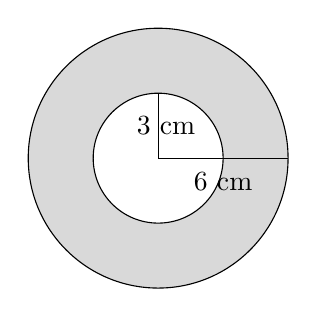
\begin{tikzpicture}[scale=0.55]
\def\R{3}
\def\r{1.5}

\fill[gray!30] (0,0) circle (\R);
\fill[white] (0,0) circle (\r);

\draw (0,0) circle (\R);
\draw (0,0) circle (\r);

\draw (0,0) -- (\R,0);
\draw (0,0) -- (0,\r);

% FIXED: Use separate coordinates for midpoint calculation
\path (0,0) -- (\R,0) coordinate[midway] (midR);
\path (0,0) -- (0,\r) coordinate[midway] (midr);
\node at (midR) [yshift=-0.3cm] {$6$ cm};
\node at (midr) [xshift=+0.1cm] {$3$ cm};
\end{tikzpicture}

\vspace{0.2cm}
Find the shaded area.

\ashow{Area = \(27\pi\text{ cm}^2\)}

\vspace{0.4cm}

\textbf{3.}

\begin{tikzpicture}[scale=0.45]

\draw (0,0) rectangle (3,2);
\node at (1.5,-0.4) {\small A};
\node at (1.5,2.5) {6};
\node at (-0.4,1) {4};

\draw (5,0) rectangle (9.5,3);
\node at (7.25,-0.4) {\small B};
\node at (7.25,3.5) {9};
\node at (4.6,1.5) {6};

\end{tikzpicture}

Find the scale factor mapping \newline A → B.

\ashow{Scale factor = \(1.5\)}

% RIGHT COLUMN
\column{0.5\textwidth}

\textbf{2.}

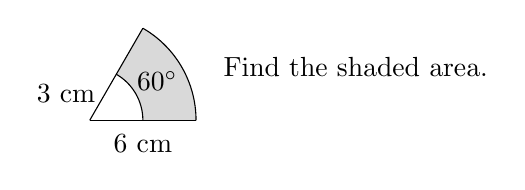
\begin{tikzpicture}[scale=0.45]
\def\R{3}
\def\r{1.5}
\def\angle{60}

% Shaded annular sector
\fill[gray!30] (0,0) -- (0:\R) arc (0:\angle:\R) -- cycle;
\fill[white] (0,0) -- (0:\r) arc (0:\angle:\r) -- cycle;

% Draw only the arcs that bound the shaded region (no full circles)
\draw (0:\R) arc (0:\angle:\R);
\draw (0:\r) arc (0:\angle:\r);

% Draw the two radii
\draw (0,0) -- (0:\R);
\draw (0,0) -- (\angle:\R);

% Labels
\node at ($(0,0)!0.5!(\R,0)$) [yshift=-0.3cm] {$6$ cm};
\node at ($(0,0)!0.5!(0,\r)$) [xshift=-0.3cm] {$3$ cm};
\node at (\angle/2:2.2) {$60^\circ$};

% Add question text to the right of the diagram
\node[anchor=west] at (3.5,1.5) {\text{Find the shaded area.}};
\end{tikzpicture}

\ashow{\(\frac{1}{6}\times 27\pi = 4.5\pi\text{ cm}^2\)}

\vspace{0.2cm}

\textbf{4.}
\begin{center}
 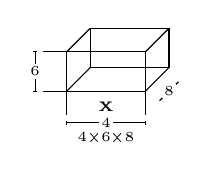
\begin{tikzpicture}[scale=0.5]
    \cuboid{0}{0}{X}{4×6×8}
\end{tikzpicture}
\end{center}

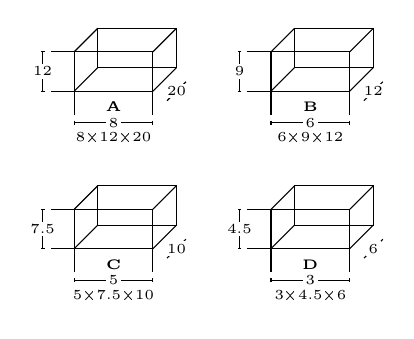
\begin{tikzpicture}[scale=0.5]
  \cuboid{0}{-2}{A}{8×12×20}
  \cuboid{5}{-2}{B}{6×9×12}
  \cuboid{0}{-6}{C}{5×7.5×10}
  \cuboid{5}{-6}{D}{3×4.5×6}
\end{tikzpicture}

Which are similar to $X$?

\ashow{Similar shapes: B, C, D}

\end{columns}

\end{frame}

%------------------------------------------------
% WORKED SOLUTIONS: STARTER 1
%------------------------------------------------

\begin{frame}{Worked Solution: Retrieve and Connect 1, Question 1}
\hypertarget{work-st1}{}

\textbf{Question:} A ring is formed by two concentric circles. The outer circle has radius \(6\) cm and the inner circle has radius \(3\) cm. Find the shaded area.

\textbf{Worked Solution:}

The shaded area is the area of the large circle minus the area of the small circle:
\[
\pi(6)^2-\pi(3)^2
=36\pi-9\pi
=27\pi.
\]
Therefore the shaded area is
\[
\boxed{27\pi\text{ cm}^2}.
\]

\end{frame}

\begin{frame}{Worked Solution: Retrieve and Connect 1, Question 2}

\textbf{Question:} A shaded annular sector has outer radius \(6\) cm, inner radius \(3\) cm, and angle \(60^\circ\). Find the shaded area.

\textbf{Worked Solution:}

The full ring has area
\[
\pi(6)^2-\pi(3)^2=27\pi.
\]

The shaded region is the sector with angle \(60^\circ\), which is
\[
\frac{60}{360}=\frac16
\]
of the full ring. Hence
\[
\text{shaded area}
=\frac16(27\pi)
=\frac{27}{6}\pi
=\frac{9}{2}\pi
=4.5\pi\text{ cm}^2.
\]
So the shaded area is
\[
\boxed{4.5\pi\text{ cm}^2}.
\]

\end{frame}

\begin{frame}{Worked Solution: Retrieve and Connect 1, Question 3}

\textbf{Question:} Rectangle \(A\) has dimensions \(6\) by \(4\). Rectangle \(B\) has dimensions \(9\) by \(6\). Find the scale factor mapping \(A\to B\).

\textbf{Worked Solution:}

The width changes from \(6\) to \(9\), so
\[
k=\frac{9}{6}=1.5.
\]
The height changes from \(4\) to \(6\), so
\[
k=\frac{6}{4}=1.5.
\]
Both dimensions are multiplied by the same factor, so the scale factor mapping \(A\) to \(B\) is
\[
\boxed{1.5}.
\]

\end{frame}

\begin{frame}{Worked Solution: Retrieve and Connect 1, Question 4}

\textbf{Question:} Cuboid \(X\) has dimensions \(4\times6\times8\). Decide which of cuboids \(A\), \(B\), \(C\), \(D\) are similar to \(X\):
\[
A=8\times12\times20,\quad B=6\times9\times12,\quad C=5\times7.5\times10,\quad D=3\times4.5\times6.
\]

\textbf{Worked Solution:}

Cuboid \(X\) has side ratio
\[
4:6:8=2:3:4.
\]
A cuboid is similar to \(X\) if its side lengths have the same ratio.

\[
\begin{array}{c|c|c|c}
\text{cuboid} & \text{dimensions} & \text{ratio} & \text{similar to }X\\ \hline
A & 8,12,20 & 2:3:5 & \text{No}\\
B & 6,9,12 & 2:3:4 & \text{Yes}\\
C & 5,7.5,10 & 2:3:4 & \text{Yes}\\
D & 3,4.5,6 & 2:3:4 & \text{Yes}
\end{array}
\]

So the cuboids similar to \(X\) are
\[
\boxed{B,\ C,\ D}.
\]

\end{frame}

\end{document}